\documentclass[12pt,letterpaper]{article}
\usepackage[left=2.00cm, right=2.00cm, top=2.00cm, bottom=2.00cm]{geometry}
\usepackage[latin1]{inputenc}
\usepackage{amsmath}
\usepackage{hyperref}
\hypersetup{
	colorlinks=true,
	linkcolor=blue,
	citecolor=magenta,      
	urlcolor=cyan,
}
\usepackage{pgfplots}
\pgfplotsset{compat=1.17}
\usepackage{amsthm}
\usepackage{amsfonts}
\usepackage{amssymb}
\usepackage{mcode} % for typesetting MATLAB code
\usepackage{graphicx}
\usepackage{framed}
\usepackage{float}
\usepackage{multicol}
\floatstyle{boxed}
\newfloat{code}{thp}{lop}
\floatname{code}{MATLAB Code}
%
% Commands for theorem environments:  For example, to typset a definition, type \begin{defn}[Definition Name] ... Definition goes here ...\end{defn}
\newtheorem{thm}{Theorem}[section]
\newtheorem{cor}[thm]{Corollary}
\newtheorem{lem}[thm]{Lemma}
\theoremstyle{definition}
\newtheorem{rem}[thm]{Remark}
\newtheorem{defn}[thm]{Definition}
\newtheorem{algorithm}[thm]{Algorithm}
\newtheorem{example}[thm]{Example}
%


\usepackage[final]{pdfpages}

\usepackage{booktabs}

\author{Daniel Ellison, DJ Poulin} % Include group member names here
\title{Jacobi and Gauss-Seidel Iterative Methods}

\begin{document}
	\maketitle 
	
\begin{abstract}
This paper introduces two stationary iterative methods for solving the matrix system of equations $A\vec{x}=b$, namely, the Jacobi and Gauss-Seidel iterative methods, which offer improved performance over the First Order Richardson and Steepest Descent methods in both number of iterations and time per iteration. These methods also demonstrate a new avenue for iterative methods, as they do not make use of the residual, unlike many other common methods. In our paper, convergence of the Jacobi and Gauss-Seidel methods for strictly diagonally dominant matrices will be proven. We will also compare and analyze the performance of the two methods, first theoretically and then as applied to the real world Model Poisson Problem (MPP). Finally, we will briefly discuss an improvement upon the Gauss-Seidel method in the form the Successive Over-Relaxtion (SOR) algorithm.
%INSERT ABSTRACT HERE

	%We will use \LaTeX to typeset our papers.  Paper length will be variable, depending on the topic of choice.  Expect papers to be, at minimum, 10 or so pages typed in size 12 font (although papers may be significantly longer, depending on what mathematics, figures, and code your topic entails).  The goal is to `tell the story' of your topic.  Think of this paper as being an expository article for a mathematical journal aimed at advanced undergraduates.
\end{abstract}

\section*{Introduction}

Iterative methods provide an efficient alternative to direct methods for solving the linear system $A\vec{x}=\vec{b}$ for $\vec{x}$ by progressively improving an approximation of $\vec{x}$ rather than exactly solving for it it. In practice, iterative methods are often created by splitting $A$ into separate matrices, for example, $A = S-T$, and then solving the resulting $S\vec{x}^{(k+1)}=T\vec{x}^{(k)}+b$ for the next iteration. While there are infinitely many ways to split $A$, only certain ones result in convergence and thus only certain ones are of any use. Two of these useful iterative methods are the Jacobi and the Gauss-Seidel methods.

Forgetting the more formal approach to iterative methods for a moment, let us consider some relatively straightforward ideas for how to improve a guessed solution to a system of linear equations. A simple approach would be to start with a guess where all the variables are equal to 0, and then continuously plugging these guesses for all but the first variable into the first equation, all but the second into the second equation, and so on. We can then compute the new value of each variable by solving each of the equations for the now single unknown, and then repeat this process with our newly calculated guess. This is actually a well-known iterative method called the Jacobi method. Jacobi first wrote about iterative methods in the early 1800s, but there was little interest in the topic until the 1960s, when the advent of computers made iterative methods more practical\cite{JacobiFirstIterativeWriting}.%1825, however, his paper was not published until 1961, when the advent of computers had brought new attention to the idea of iterative methods. \textbf{NEED CITATION}

One idea to perhaps improve this technique would be to plug the variable guesses into a single equation at a time, solve that equation, and then update the corresponding guessed variable, so that the next equation can use the updated guess for that variable (in contrast to the Jacobi Method, where we use the same guess for all the equations). This iterative method is called the Gauss-Seidel Method, although it was ``apparently unknown to Gauss and not recommended by Seidel"\cite{Strang06}. 
%Finally another intuitive idea would be to calculate the change in our guess (using either of the methods above) and then updating our guess by adding a multiple of that change with the thought that if the guess is moving in the right direction why not go even further in that correct direction. This idea is captured in a more advance iterative method called Successive Over-Relaxation (SOR) which we will touch lightly on later. One can then simply repeat any of these processes until the resulting guess is satisfactorily close enough to the true solution often determined by computing the residual. 

These methods, as we will see, are not guaranteed to quickly provide a usable answer, and indeed only converge to the true solution for specific types of linear systems. 
In this paper we will introduce both the Jacobi and Gauss-Seidel algorithms in more detail, providing practical examples and pseudo-code implementation along the way. We will also prove aspects of convergence before analyzing performance. Specifically, we will consider asymptotic and average rates of convergence. We will then apply an implementation of the Jacobi and Gauss-Seidel methods to the 1-dimensional and 2-dimensional Model Poisson Problems, comparing performance to Gaussian Elimination. Finally, in our conclusion, we will discuss avenues of improvement for the two algorithms, namely the Successive Over-Relaxation (SOR) algorithm, a slight variation on these methods which is considerably more powerful.


\section{Explanation of Algorithms}
We now begin by introducing the two algorithms more formally and with numerical examples, which we calculate ``by hand."
%We will introduce both algorithms in an intuitive manner using sample linear equations to perform some iterations ``by hand" and simultaneously introduce the matrix notation we will use for the rest of the paper. This section should leave the reader with a solid understanding of both methods and how to actually carry them out. 
\subsection{Jacobi Method}

Let us now more formally introduce the Jacobi method. Recall from the introduction that, intuitively, this method is plugging in all but one of our guesses for the variables into each of the linear equations and then computing the now single unknown in each equation. We will set our initial guess to be the zero vector. Following the explanation from Strong \cite{Strong05}, for an $n\times n$ matrix $A$, we can describe this iterative improvement as

\begin{equation}\label{jacobi_intro}
    \begin{matrix}
    a_{11}x_1^{(k+1)}&+&a_{12}x_2^{(k)}&+&\cdots&+&a_{1n}x_n^{(k)}&=&b_1\\
    a_{21}x_1^{(k)}&+&a_{22}x_2^{(k+1)}&+&\cdots&+&a_{2n}x_n^{(k)}&=&b_2\\
    \vdots &&\vdots &&\vdots &&\vdots&&\vdots\\
    a_{n1}x_1^{(k)}&+&a_{n2}x_2^{(k)}&+&\cdots&+&a_{nn}x_n^{(k+1)}&=&b_n\\
    \end{matrix},
\end{equation}

\noindent where the $x^{(k+1)}$ terms will become our improved guess values, and the $x^{(k)}$ terms are our current iteration's guesses. We can thus solve for the $x^{(k+1)}$ terms, as all other terms are known (either constants like $b$ or our current guess values $x^{(k)}$). Solving for these terms leads us to the linear form of the Jacobi method, namely,

\begin{defn}{Linear Form of the Jacobi Method}
\begin{equation*}
    x_i^{(k+1)}=\frac{b_i-\sum\limits_{j=1,j\neq i}^n a_{ij}x_j^{(k)}}{a_{ii}}.
\end{equation*}

\end{defn}

\noindent It is worth noting that we can calculate $x_i^{(k+1)}$ for any $i$ without knowledge of any other $x_i^{(k+1)}$ values. However, it will be more useful to express this iteration in matrix form. Looking at equation \ref{jacobi_intro}, we see the $(k+1)$ terms are always paired with $a_{i,i}$ and so we can rewrite equation \ref{jacobi_intro} as $$D\vec{x}^{(k+1)} + (L+U)\vec{x}^{(k)} = \vec{b},$$ where $L$ equals the lower triangular portion of $A$, $U$ equals the upper triangular portion, and $D$ equals the diagonal such that $A=U+L+D$. Solving for $\vec{x}^{(k+1)}$ yields the matrix iteration: 

\begin{defn}[Matrix Form of the Jacobi Method]
$$\vec{x}^{(k+1)}=D^{-1}\left[\vec{b}-(L+U)\vec{x}^{(k)}\right]$$
\end{defn}

\begin{example}
Let us solve $A\vec{x}=\vec{b}$ using the Jacobi method where 
\begin{equation}\label{sample_axb}
A=
    \begin{bmatrix}
    7 & 1 & 3 & 2\\
    2 & 5 & 1 & 1\\
    4 & 3 & 10 & 2\\
    1 & 8 & 2 & 12
    \end{bmatrix}, 
%x_{true} =
%\begin{bmatrix}
%1\\-1\\2\\-3
%\end{bmatrix},
\vec{b}=
\begin{bmatrix}
6\\-4\\15\\-39
\end{bmatrix},
\vec{x}^{(0)} =
\begin{bmatrix}
0\\0\\0\\0
\end{bmatrix}.
\end{equation}

For maximum clarity, we will make substitutions into the linear equations rather than use the linear form of the Jacobi Method. Then we write

\begin{equation*}
    \begin{matrix}
    7x_1^{(k+1)} &+& 1x_2^{(k)} &+& 3x_3^{(k)} &+& 2x_4^{(k)} &=& 6\\
    2x_1^{(k)} &+& 5x_2^{(k+1)} &+& 1x_3^{(k)} &+& 1x_4^{(k)} &=& -4\\
    4x_1^{(k)} &+& 3x_2^{(k)} &+& 10x_3^{(k+1)} &+& 2x_4^{(k)} &=& 15\\
    1x_1^{(k)} &+& 8x_2^{(k)} &+& 2x_3^{(k)} &+& 12x_4^{(k+1)} &=& -39
    \end{matrix}.
\end{equation*}

For $k=0$, $\vec{x}^{(0)}=\vec{0}$, so we have
\begin{equation*}
    \begin{array}{ccccccccc|l}
    7x_1^{(1)} &+& 1(0) &+& 3(0) &+& 2(0) &=& 6& x_1^{(1)}=6/7 \\
    2(0) &+& 5x_2^{(1)} &+& 1(0) &+& 1(0) &=& -4&  x_2^{(1)}=-4/5\\
    4(0) &+& 3(0) &+& 10x_3^{(1)} &+& 2(0) &=& 15& x_3^{(1)}=15/10 \\
    1(0) &+& 8(0) &+& 2(0) &+& 12x_4^{(1)} &=& -39& x_4^{(1)}=-39/12
    \end{array}.
\end{equation*}

We get the same result using the matrix form of the Jacobi method:
\begin{equation*}
    \vec{x}^{(k+1)} = \begin{bmatrix}1/10&0&0&0\\0&1/5&0&0\\0&0&1/10&0\\0&0&0&1/12
    \end{bmatrix}\left(\begin{bmatrix}6\\-4\\15\\-39\end{bmatrix}- \begin{bmatrix}
    0 & 1 & 3 & 2\\
    2 & 0 & 1 & 1\\
    4 & 3 & 0 & 2\\
    1 & 8 & 2 & 0
    \end{bmatrix}\begin{bmatrix}
0\\0\\0\\0
\end{bmatrix}\right)=\begin{bmatrix}
6/7\\-4/5\\15/10\\-39/12
\end{bmatrix}
\end{equation*}
The results of this iteration and selected subsequent iterations are below.\\

\begin{tabular}{crrrrrrrr}
     \toprule
    Iteration & 0 & 1 & 2 & 3 & 4 & 5 & 50 & True Solution \\
    \midrule
    $x_1$ & 0 & .8571 & 1.2571 & .9611 & 1.1302 & .9257 & 1.0001 & 1\\
    $x_2$ & 0 & -.800 & -.7929 & -1.1047 & -.9195 & -1.0880 & -.9999 & -1\\
    $x_3$ & 0 & 1.500 & 2.0471 & 1.8426 & 2.0804 & 1.9039 & 2.0001 & 2\\
    $x_4$ & 0 & -3.25 & -3.0381 & -3.1674 & -2.9007 & -3.0779 & -2.9999 & -3\\
    \bottomrule
\end{tabular}
\begin{center}
    \it Results from selected iterations of the Jacobi method.
\end{center}
\end{example}

\subsection{Gauss-Seidel Method}
The Gauss-Seidel method improves on the Jacobi method by using the updated guess values as we go down the equations. For instance, after we solve the first equation we have a value for $x_1^{(k+1)}$ we can use in the following equations instead of the $x_1^{(k)}$ we continued using in the Jacobi method. The same is true for the $x_2^{(k+1)}$ value after solving the second equation, and so on. We can thus rewrite our iterative improvement in terms of linear equations as\cite{Strong05}:

\begin{equation}
    \begin{matrix}
    a_{11}x_1^{(k+1)}&+&a_{12}x_2^{(k)}&+&\cdots&+&a_{1n}x_n^{(k)}&=&b_1\\
    a_{21}x_1^{(k+1)}&+&a_{22}x_2^{(k+1)}&+&\cdots&+&a_{2n}x_n^{(k)}&=&b_2\\
    \vdots &&\vdots &&\vdots &&\vdots&&\vdots\\
    a_{n1}x_1^{(k+1)}&+&a_{n2}x_2^{(k+1)}&+&\cdots&+&a_{nn}x_n^{(k+1)}&=&b_n
    \end{matrix}
\end{equation}

\noindent Once again we set the initial guess to be the zero vector. As before we can isolate the $(k+1)$ terms to arrive at the linear form.

\begin{defn}{(Linear Form of the Gauss-Seidel Method)}
\begin{equation*}
    x_i^{(k+1)} = \frac{b_i-\sum\limits_{j=1}^{i-1}a_{ij}x_j^{(k+1)}-\sum\limits_{j=i+1}^{n}a_{ij}x_j^{(k)}}{a_{ii}}
\end{equation*}
\end{defn}

In the Gauss-Seidel method, we must solve for each $x_i^{(k+1)}$ sequentially, as to do so requires knowledge of all the previous $x_i^{(k+1)}$ values. Looking at the linear equations as a matrix we see we have only changed the terms in the lower triangular portion from $(k)$ to $(k+1)$, and so we can express it as $$L\vec{x}^{(k+1)}+D\vec{x}^{(k+1)}+U\vec{x}^{(k)}=\vec{b}.$$ 

\noindent This leads us to our matrix definition of the Gauss-Seidel method:
\begin{defn}(Matrix Form of Gauss-Seidel Method)
$$\vec{x}^{(k+1)} = (L+D)^{-1}\left(\vec{b}-U\vec{x}^{(k)}\right).$$
\end{defn}
\begin{example}

Using the same $4\times4$ example from equation \ref{sample_axb} we have

\begin{equation*}
    \begin{matrix}
    7x_1^{(k+1)} &+& 1x_2^{(k)} &+& 3x_3^{(k)} &+& 2x_4^{(k)} &=& 6\\
    2x_1^{(k+1)} &+& 5x_2^{(k+1)} &+& 1x_3^{(k)} &+& 1x_4^{(k)} &=& -4\\
    4x_1^{(k+1)} &+& 3x_2^{(k+1)} &+& 10x_3^{(k+1)} &+& 2x_4^{(k)} &=& 15\\
    1x_1^{(k+1)} &+& 8x_2^{(k+1)} &+& 2x_3^{(k+1)} &+& 12x_4^{(k+1} &=& -39
    \end{matrix}.
\end{equation*}

For $k=0$, $x^{(0)}=\vec{0}$, we can write
\begin{equation*}
    \begin{array}{ccccccccc|l}
    7x_1^{(1)} &+& 1(0) &+& 3(0) &+& 2(0) &=& 6 & x_1^{(1)}=6/7 \\
    2(6/7) &+& 5x_2^{(1)} &+& 1(0) &+& 1(0) &=& -4 & x_2^{(1)}=-8/7\\
    4(6/7) &+& 3(-8/7) &+& 10x_3^{(1)} &+& 2(0) &=& 15& x_3^{(1)}=3/2 \\
    1(6/7) &+& 8(-8/7) &+& 2(3/2) &+& 12x_4^{(1} &=& -39& x_4^{(1)}=-59/21
    \end{array}
\end{equation*}

We can get the same result with the matrix form as well:
\begin{equation*}
    x^{(k+1)}=\begin{bmatrix}
    7 & 0 & 0 & 0\\
    2 & 5 & 0 & 0\\
    4 & 3 & 10 & 0\\
    1 & 8 & 2 & 12
    \end{bmatrix}^{-1}\left(  \begin{bmatrix}6\\-4\\15\\-39\end{bmatrix} -\begin{bmatrix}
    0 & 1 & 3 & 2\\
    0 & 0 & 1 & 1\\
    0 & 0 & 0 & 2\\
    0 & 0 & 0 & 0
    \end{bmatrix}\begin{bmatrix}
0\\0\\0\\0
\end{bmatrix}\right)=\begin{bmatrix}
6/7\\-8/7\\3/2\\-59/21
\end{bmatrix}
\end{equation*}

The results of this iteration and selected subsequent iterations are below. Note that the Gauss-Seidel method appears to converge significantly faster than the Jacobi method. This will be discussed in more depth in a later section.\\

\begin{tabular}{crrrrrrrr}
     \toprule
    Iteration & 0 & 1 & 2 & 3 & 4 & 5 & 6 & True Solution \\
    \midrule
    $x_1$ & 0 & .8571 & 1.1803 & 1.0446 & 1.0089 & 1.0016 & 1.0003 & 1\\
    $x_2$ & 0 & -1.1429 & -1.0102 & -.9983 & -.9992 & -.9998 & -1.0000 & -1\\
    $x_3$ & 0 & 1.5000 & 1.8929 & 1.9797 & 1.9965 & 1.9994 & 1.9999 & 2\\
    $x_4$ & 0 & -2.8095 & -2.9904 & -3.0014 & -3.0007 & -3.0002 & -3.0000 & -3\\
    \bottomrule
\end{tabular}
\begin{center}
    \it Results from selected iterations of the Gauss-Seidel method.
\end{center}
For comparison, the 50th iteration of the Jacobi method is $\begin{bmatrix}1.0001&-.9999&2.0001&-2.9999\end{bmatrix}^T$, which is comparable to the 6th iteration of the Gauss-Seidel method.

\end{example}


\subsection{MATLAB Implementation}

%(TODO: BETTER EXPLANATIONS FOR WHAT IS GOING ON. PERFORMANCE IMPROVEMENTS?)

Considering the computational complexity of these algorithms, especially as the dimensions of our linear system get larger, we would rather not always compute the results by hand. Certainly, any practical implementation of the Jacobi and Gauss-Seidel methods would implement the algorithms via programming rather than by hand. As such, we have included a pseudo-code implementation of each method. For a MATLAB implementation, see the appendix at the end of our paper.
%As such, we have included a MATLAB implementation of each method to show how they can be used by a computer.

%\subsection{Jacobi Method in MATLAB}

%While the MATLAB implementation of the Jacobi method looks similar to how we outlined the algorithm above, a few changes have been made in the name of performance. Namely, we calculate a few constants before beginning the iterative method, such as $D^{-1}$, so that we do not have to calculate them in every iteration.

% NOTE: I changed the MATLAB slightly -Dan
%This function implements the Jacobi method.
%A and b are the knowns in Ax = b.
%xGuess is our starting guess. If nothing is known about x, use the zero
%vector
%tol is the desired upper bound for the relative residual
%itMax is the maximum number of iterations our algorithm will go through

%To save some calculations during the for loop, we calculate
%the norm of b, the inverse of D, and L plus U here.
%First, we initialize L, U, D, and xold (our starting guess for x)
%Here, we implement the Jacobi method itself
 %We check if the desired relative residual has been reached. If so, we
    %return. Otherwise, we continue
    
    %If we reach the max number of iterations, we return what we have so far as
%well as the current relative residual. We also let the user know that we
%have reached the max number of iterations.
%disp('We have reached the max number of iterations,')
%disp('but we have not reached the desired tolerance (relative residule)')
%U = A - tril(A);
%D = diag(diag(A));

\begin{algorithm}[Jacobi Method]
\footnotesize
\begin{verbatim}

inputs: A, b, xOld, itMax
L = lower triangular portion of A
U = upper triangular portion of A
D = diagonal portion of A
for iteration = 1:itMax
    xNew = inv(D) * (b - (L + U) * xOld)
    check for convergence
    xOld = xNew
\end{verbatim}
\end{algorithm}
%\begin{algorithm}[Jacobi Method]
%\begin{lstlisting}
%
%function [xnew, i] = Jacobi(A, b, xGuess, tol, itMax)
%L = tril(A, -1);
%LplusU = A - D;
%xold = xGuess;
%bNorm = norm(b);
%DInverse = inv(D);
%LplusU = L+U;
%for i = 1:itMax
%    xnew = DInverse * (b - LplusU * xold);
%    xold = xnew;
%    relativeResidual = norm(b - A * xnew, 2) / bNorm;
%    if  relativeResidual <= tol
%        return
%    end
%end
%end
%\end{lstlisting}
%\end{algorithm}
%\subsection{Gauss-Seidel Method in MATLAB}

%Again, the algorithm looks almost exactly like our above explanation of the Gauss-Seidel method. We once more calculate constants before beginning the iterative method to save on operations. These algorithms also illustrate how similar the Jacobi and Gauss-Seidel methods are; the for loops are identical aside from the calculation of xnew, which is only slightly different in the two methods.

%This function implements the Gauss-Seidel method.
%A and b are the knowns in Ax = b.
%xGuess is our starting guess. If nothing is known about x, use the zero
%vector
%tol is the desired upper bound for the relative residual
%itMax is the maximum number of iterations our algorithm will go through

%First, we initialize L, U, D, and xold (our starting guess for x)

%To save some calculations during the for loop, we calculate
%the norm of b and the inverse of L + D.


%Here, we implement the Gauss-Seidel method itself
 %We check if the desired relative residual has been reached. If so, we
    %return. Otherwise, we continue
    %If we reach the max number of iterations, we return what we have so far as
%well as the current relative residual. We also let the user know that we
%have reached the max number of iterations.
%disp('We have reached the max number of iterations,')
%disp('but we have not reached the desired tolerance (relative residule)')
\begin{algorithm}[Gauss-Seidel]
\footnotesize
\begin{verbatim}

inputs: A, b, xOld, itMax
L = lower triangular portion of A
U = upper triangular portion of A
D = diagonal portion of A
for iteration = 1:itMax
    xNew = inv(L + D) * (b - U * xold)
    check for convergence
    xOld = xNew
\end{verbatim}
%\begin{lstlisting}
%
%function [xnew, i] = GS(A, b, xGuess, tol, itMax)
%L = tril(A, -1);
%U = A - tril(A);
%D = diag(diag(A));
%xold = xGuess;
%bNorm = norm(b);
%LplusDInverse = inv(L + D);
%for i = 1:itMax
 %   xnew = LplusDInverse * (b - U * xold);
  %  xold = xnew;
   % relativeResidual = norm(b - A * xnew, 2) / bNorm;
    %if  relativeResidual <= tol
     %   return
%    end
%end
%end
%\end{lstlisting}
\end{algorithm}

\section{Convergence Analysis}
%(TODO IMPROVE FORMATTING, CLARITY. GAUSS-SEIDEL PROOF. CITATIONS. PROVE THM 3.2?)

While the Jacobi and Gauss-Seidel methods certainly have their strengths, we are by no means guaranteed a usable result from either of them. For many linear systems $A\vec{x} = \vec{b}$, the iterative methods will diverge, such that our final result will tell us nothing about the true value of $\vec{x}$. It would therefore be useful to know whether these methods will converge for a given linear system before we spend the time and storage calculating iterations. There are a number of criteria that guarantee convergence for each method. Below, we outline a few such criteria.

\subsection{General Convergence for Fixed-Point Iterations}
Both the Jacobi and Gauss-Seidel methods are fixed-point iterations. Fixed-point iterations can be written in the form of $\vec{x}^{(k)} = T\vec{x}^{(k-1)} + \vec{c}$, where $T$ is called the iteration matrix. We would like a theorem that works for iterative methods of this form, as it would apply to both the Jacobi and Gauss-Seidel methods. We will therefore prove the following theorem.

%Iterative methods of this form converge when $\rho(T) < 1$. We will use this result to find other convergence criteria for the Jacobi and the Gauss-Seidel Methods, but we first need to prove it.

\begin{thm}\label{rho(t) < 1}
An iterative method of the form $\vec{x}^{(k)} = T\vec{x}^{(k-1)} + \vec{c}$, with $T$ the iteration matrix, will converge if and only if $\rho(T) < 1$.
\end{thm}


\noindent Our proof of this will involve finding a way to write $\vec{x}^{(n)}$ in terms of $T$, and then showing that these terms of $T$ converge. For this purpose, we will accept a few results, namely Lemma \ref{lemma General Convergence Proof} and Theorem \ref{toinf, rho(A)<1}. We omit proofs of these, as we will focus more on results specific to the Jacobi and GS methods. We refer the interested reader to \cite{Keller} for more details.

\begin{lem}\label{lemma General Convergence Proof}
If the spectral radius satisfies $\rho(T) < 1$, then $(I-T)^{-1}$ exists and equals 
\\$I + T + T^{2} + ... = \sum_{n=0}^{\infty} T^{n}$.
\end{lem} 

Once we have $\vec{x}^{(n)}$ written in terms of $T$, we will take the limit of both sides. Lemma \ref{lemma General Convergence Proof} will allow us to state that this limit exists, which in turn will allow us to state that our method converges. This will be the last step of our proof, so if this seems a bit abstract right now, it should become more understandable as we continue.


\begin{thm}\label{toinf, rho(A)<1}
The following statements are equivalent.
\\1) $\rho{(T)}<1$.
\\2) $\lim_{n\to\infty} ||T^{n}|| = 0$ for some natural induced matrix norm $||\medspace||$.
\\3) $\lim_{n\to\infty}T^n\vec{x} = 0$ for every $\vec{x}$.
\end{thm}

Theorem \ref{toinf, rho(A)<1} will also be useful once we write $\vec{x}^{(n)}$ in terms of $T$, as it, too, will help us show a limit exists. Also, since Theorem \ref{toinf, rho(A)<1} gives us a way of confirming $\rho{(T)} < 1$, we can use it to help prove the converse of Theorem \ref{rho(t) < 1} - namely, that convergence of our iterative method implies $\rho{(T)} < 1$. We define the concept of a natural norm, which this theorem references, below.

\begin{defn}
$||\medspace||$ is a natural matrix norm if $||\medspace||$ is an induced matrix norm and, for some matrix $B$, $||B|| = \max_{|z| = 1}||A\vec{z}||$.
\end{defn}

In regards to this definition, it should be noted that the definition of a natural matrix norm is only tangentially important to the topic at hand; more important is the understanding that the infinity norm is a natural norm, so, by Theorem \ref{toinf, rho(A)<1}, if $||A||_\infty<1$, then $\rho{(A)}<1$. For further reading on natural norms in general, see \cite{Natural_Norms}.

%\begin{proof}
%Let $\rho(T) < 1$, and let $(\lambda, \vec{x})$ be an eigenpair of T. Then $T\vec{x} = \lambda\vec{x}$, so we can write 
%$$\vec{x} - T\vec{x} = \vec{x} - \lambda\vec{x},$$ which is equivalent to $$(I - T)\vec{x} = (1 - \lambda)\vec{x}.$$ Then if $\lambda$ is an eigenvalue of $T$, $(1 - \lambda)$ is an eigenvalue of $(I - T)$. Since $|\lambda| \leq \rho(T) < 1$, $\lambda$ cannot equal 1. Then $(1 - \lambda) \geq 0$, so 0 cannot be an eigenvalue of $(I - T)$. Then we know that $(I - T)^{-1}$ exists.

%Now, let the matrix $$S_m = I + T + T^2 + ... + T^m.$$ Multiply by $(I - T)$ on the left to get 
%\begin{align*}(I - T)S_m &= (I + T + T^2 + ... + T^m) - (T + T^2 + T^3 + ... + T^{m+1})
%\\&=I - T^{m + 1}.\end{align*} \textbf{Since T is convergent, $(I - T)$ is convergent}. Take the limit of both sides to get $$\lim_{m\to\infty}(I - T)S_m = \lim_{m\to\infty}I - T^{m+1},$$ which is equivalent to $$(I - T)\lim_{m\to\infty}S_m = I - \lim_{m\to\infty}T^{m+1}.$$ \textbf{Then, by theorem }\ref{toinf},$$(I - T)\lim_{m\to\infty}S_m = I - \lim_{m\to\infty}T^{m+1} = I.$$ Multiply both sides by $(I - T)^{-1}$ on the left to get $$\lim_{m\to\infty}S_m = I - T.$$ So, $$(I - T)^{-1} = I + T + T^2 + ... = \sum_{n=0}^{\infty} T^{n}.$$ This proves the desired lemma.
%\end{proof}


With these results, we can begin our proof of Theorem \ref{rho(t) < 1}. This proof follows and elaborates on the proof from \cite{Burden}, specifically the proof from the ``Convergence Results for General Iteration Methods" section.

\noindent \textit{Proof.} 
Assume that $\rho(T) < 1$. Recall that in iterative methods we define $\vec{x}^{(k)}$ with 
$$\vec{x}^{(k)} = T\vec{x}^{(k-1)} + \vec{c}.$$ Since 
$$\vec{x}^{(k-1)} = T\vec{x}^{(k-2)} + \vec{c},$$ we have, via substitution, 
\begin{align*}\vec{x}^{(k)} &= T\left(T\vec{x}^{(k-2)} + \vec{c}\right) + \vec{c}
%= T^{2}\vec{x}^{(k-2)} + T\vec{c} + \vec{c}\end{align}
\\&= T^{2}\vec{x}^{(k-2)} + (T + I)\vec{c}.
\\&= T^{2}\left(T\vec{x}^{(k-3)} + \vec{c}\right) + (T + I)\vec{c} 
\\&= T^{3}\vec{x}^{(k-3)} + (T^2 + T + I)\vec{c}.\end{align*} 
We can continue substituting in this way until we are left with 

\begin{align*}\vec{x}^{(k)} = T^{k}\vec{x}^{(0)} + \left(T^{k-1} + ... + T + I\right)\vec{c}.\end{align*} Take the limit of both sides to get 
\begin{align*}\lim_{k\to\infty}\vec{x}^{(k)} =& \lim_{k\to\infty}T^{k}\vec{x}^{(0)} + \left(T^{k-1} + ... + T + I\right)\vec{c}. 
\\ =& \lim_{k\to\infty}T^{k}\vec{x}^{(0)} + \lim_{k\to\infty}\left(T^{k-1} + ... + T + I\right)\vec{c}.\end{align*} 

\noindent Since $\rho(T) < 1$, by Theorem \ref{toinf, rho(A)<1},  $\lim_{k\to\infty}T^{k}x^{(0)} = 0$. Then we have 

$$\lim_{k\to\infty}\vec{x}^{(k)} = \lim_{k\to\infty}\left(T^{k-1} + ... + T + I\right)\vec{c}.$$ 

\noindent By Lemma \ref{lemma General Convergence Proof}, %\begin{align*}
$$\lim_{k\to\infty}\left(T^{k-1} + ... + T + I\right)\vec{c} = \left(\sum_{n=0}^{\infty} T^{n}\right)\vec{c}= (I - T)^{-1}\vec{c}.$$
%\\&= (I - T)^{-1}\vec{c}.\end{align*} 
Then we have shown \begin{align*}\lim_{k\to\infty}\vec{x}^{(k)} = (I - T)^{-1}\vec{c}.\end{align*} 

This is the result we are looking for, though the notation is a bit different than what we might be used to. By proving the existence of this limit, we have shown that, when $\rho(T) < 1$, our approximations of $\vec{x}$ converges to a single vector, which means the iterative method converges.

We still need to show that the converse is true, namely, that convergence of the iterative method implies $\rho(T) < 1$. To do this, we will define the error of an iteration.

\begin{defn}
The error vector, $\vec{e}$, of the $k$th iteration is defined as $\vec{e}^{(k)} = \vec{x} - \vec{x}^{(k)}$. If an iterative method converges, then the error of the iterative method converges to 0.
\end{defn}

%mportant to proving more specific criterion for the Jacobi and Gauss-Seidel Methods. To do this, 
\noindent We will now prove that convergence of our iterative methods implies $\rho(T) < 1$. Assume $\vec{x}^{(k)}$ converges to $\vec{x}$. Then \begin{align}\vec{x} = T\vec{x} + \vec{c}.\end{align} 
%\noindent Consider the $0$th error, $\vec{e}^{(0)} = \vec{x} - \vec{x}^{(0)}$. 
%Then
%\begin{align*}\vec{x}^{(0)} = \vec{x} - \vec{e}^{(0)}.\end{align*} 
\noindent Recall that \begin{align}\vec{x}^{(k)} = T\vec{x}^{(k-1)} + \vec{c}.\end{align}  

\noindent Subtract equation 5 from equation 4 to get 
\begin{align*}\vec{x} - \vec{x}^{(k)} &= (T\vec{x} + \vec{c}) - \left(T\vec{x}^{(k-1)} + \vec{c}\right) 
\\&= T\left(\vec{x} - \vec{x}^{(k-1)}\right)\end{align*}
which is equivalent to
\begin{align} \vec{e}^{(k)} = T\vec{e}^{(k-1)}.\end{align}
Equation 6 reveals a relationship between $\vec{e}^{(k)}$ and $\vec{e}^{(k-1)}$ that we will now manipulate. We apply this relationship to equation 6 itself to get
\begin{align*} \vec{e}^{(k)} &= T(T\vec{e}^{(k-2)}) \\&= T^2\vec{e}^{(k-2)}.\end{align*}

%\noindent We can combine equations (6), (7), and (9) to get
%\begin{align*}\vec{x} - \vec{x}^{(k)} &= T\left(T\vec{x} + \vec{c} - \left(T\vec{x}^{(k-2)} + \vec{c}\right)\right)
%\\&= T^2\left(\vec{x} - \vec{x}^{(k-2)}\right).\end{align*} 

\noindent We can repeat this process until we are left with \begin{align*}\vec{e}^{(k)} = T^{k}\vec{e}^{(0)}.\end{align*} 
%Since $\vec{z} = \vec{x} - \vec{x}^{(0)}$, we have \begin{align*}\vec{x} - \vec{x}^{(k)} = T^{k}\vec{z}.\end{align*} 
\noindent Take the limit of both sides to get \begin{align*}\lim_{k \to \infty}\vec{e}^{(k)} = \lim_{k \to \infty}T^{k}\vec{e}^{(0)}.\end{align*} Since we assumed our iterative method converges, $\lim_{k \to \infty}\vec{e}^{(k)} = 0$. So \begin{align*}\lim_{k \to \infty}T^{k}\vec{e}^{(0)} = 0.\end{align*} 
\noindent Since $\vec{e}^{(0)}$ is a fixed vector not equal to $\vec{0}$, we know that $\lim_{k \to \infty}T^{k}$ must equal $0$. Then, by Theorem \ref{toinf, rho(A)<1}, $\rho(T)<1$. This proves the converse of Theorem \ref{rho(t) < 1}.

%\subsection{A Sufficient Condition for Convergence}
%Before we get into the Jacobi and Gauss-Seidel methods more specifically, we prove one more condition for convergence. 
%\begin{thm}\label{some norm < 1}
%If $||T||<1$ for some induced matrix norm, than the iterative method $\vec{x}^{(k)} = T\vec{x}^{(k-1)} + \vec{c}$ converges.
%\end{thm}




\subsection{Jacobi Method}
%We will prove that the Jacobi Method converges when the iteration matrix has a spectral radius, or a 2-norm, of less than one. We will also prove that if the matrix A is diagonally dominant, then the Jacobi Method will converge. Finally, we will mention that both of these theorems only go one way, and that the Jacobi method might still converge even if none of the conditions of these theorems are met.

Armed with Theorem \ref{rho(t) < 1}, we can now find more specific, less expensive criteria for the convergence of the Jacobi and Gauss-Seidel methods. While Theorem \ref{rho(t) < 1} is a powerful result on its own, eigenvalues are expensive to calculate, so we would prefer a convergence criteria that we can more easily check. For that reason, we will prove Theorem \ref{Jacobi GS Convergence Thm}.

\begin{thm}\label{Jacobi GS Convergence Thm}When A is strictly row dominant, 1) the Jacobi method converges, and 2) the Gauss Seidel method converges.\end{thm} 

Since we already have Theorem \ref{rho(t) < 1}, we only need to prove that strict row dominance of $A$ implies $\rho(T) < 1$, and then we can apply Theorem \ref{rho(t) < 1}. Because row dominance (defined below) is relatively inexpensive to check for, Theorem \ref{Jacobi GS Convergence Thm} will be more practical for checking convergence.

\begin{defn}\label{Strictly Row Dominant Matrices}
A square matrix $A$ of size $n$ is strictly row dominant if, for all rows, the absolute value of the diagonal entry is greater than the sum of absolute values of the other entries. That is to say, every row $i$ satisfies $|a_{i,i}| > |a_{i,1}| + ... + |a_{i,i-1}| + |a_{i,i+1}| + ... + |a_{i,n}|$.
\end{defn}
\noindent We will now prove part (1) of Theorem \ref{Jacobi GS Convergence Thm}. The following proof paraphrase and elaborates on the proof on page 477 of \cite{Ford15}.
\begin{proof}
Assume A is strictly row dominant. Recall the matrix form of the Jacobi method, $$\vec{x}^{(k+1)}=D^{-1}\left[\vec{b}-(L+U)\vec{x}^{(k)}\right],$$ which can be rewritten as $$\vec{x}^{(k+1)} = D^{-1}\vec{b} - D^{-1}(L + U)\vec{x}^{(k)}.$$ Then, for the true solution $\vec{x}$, we can write $$\vec{x} = D^{-1}\vec{b} - D^{-1}(L + U)\vec{x}.$$ For better notation, let $T_{J} = -D^{-1}(L + U)$ and $\vec{c}_{J} = D^{-1}\vec{b}$ so that $\vec{x} = T_{J}\vec{x} + \vec{c}_J$. %Recall that $\vec{x}^{(k+1)}=D^{-1}\left[b-(L+U)\vec{x}^{(k)}\right]$. Then we can write $\vec{x}^{(k+1)} = B_{J}\vec{x}^{(k)} + c_J$.
Note that $T_J = -D^{-1}(L + U)$ is the iteration matrix for the Jacobi method, which means $T_J$ is the matrix we would like to show satisfies $\rho(T_J) < 1$. Recall that $D$ is the main diagonal of $A$, that $L$ is the lower triangular portion of $A$, and that $U$ is the upper triangular portion of $A$. Since $D$ is the diagonal, we can write that %$-D^{-1} = $

 %   $$-D^{-1} =\begin{bmatrix}
  %  -\frac{1}{a_{11}} & 0 & \cdots & 0\\
   % 0 & -\frac{1}{a_{22}} & \cdots & 0\\
    %\vdots & \vdots & \ddots & \vdots\\
    %0 & 0 & \cdots & -\frac{1}{a_{nn}}\\
    %\end{bmatrix}.$$
    
%Then $T_J = -D^{-1}(L + U) = $

    \begin{align*}
    %%
    -D^{-1} &=\begin{bmatrix}
    -\frac{1}{a_{11}} & 0 & \cdots & 0\\
    0 & -\frac{1}{a_{22}} & \cdots & 0\\
    \vdots & \vdots & \ddots & \vdots\\
    0 & 0 & \cdots & -\frac{1}{a_{nn}}\\
    \end{bmatrix},\\
    T_J = -D^{-1}(L + U) &=\begin{bmatrix}
    -\frac{1}{a_{11}} & 0 & \cdots & 0\\
    0 & -\frac{1}{a_{22}} & \cdots & 0\\
    \vdots & \vdots & \ddots & \vdots\\
    0 & 0 & \cdots & -\frac{1}{a_{nn}}\\
    \end{bmatrix}
    \begin{bmatrix}
    0 & a_{12} & \cdots & a_{1n}\\
    a_{21} & 0 & \cdots & a_{2n}\\
    \vdots & \vdots & \ddots & \vdots\\
    a_{n1} & a_{n2} & \cdots & 0\\
    \end{bmatrix}
    \\&=\begin{bmatrix}
    0 & -\frac{a_{12}}{a_{11}} & \cdots & -\frac{a_{1n}}{a_{11}}\\
    -\frac{a_{21}}{a_{22}} & 0 & \cdots & -\frac{a_{2n}}{a_{22}}\\
    \vdots & \vdots & \ddots & \vdots\\
    -\frac{a_{n1}}{a_{nn}} & \frac{a_{n2}}{a_{nn}} & \cdots & 0\\
    \end{bmatrix}.\end{align*}
    
We will now show that $||T_{J}||_{\infty} < 1$. This will imply that $\lim_{k\to\infty}||T_{J}||_{\infty}^k = 0$, a fact that will in turn allow us to show that $\rho{(T)} < 1$. While the reasoning behind this might not be immediately clear, it will become clearer as we continue the proof. Recall that the infinity norm is the maximum row sum. Then, by definition,
\begin{align*}||T_{J}||_{\infty} = \max_{1\leq i\leq n}\sum_{j=1}^{n}|T_{J_{ij}}|.\end{align*} Notice that all the diagonal elements of $T_{J}$ equal $0$. Then \begin{align*}||T_{J}||_{\infty} = \max_{1\leq i\leq n}\left[\sum_{j=1:j\neq i}^{n}|T_{J_{ij}}|\right].\end{align*} We have already calculated $T_{J_{ij}} = -\frac{a_{ij}}{a_{ii}}$, so 

\begin{align*}||T_{J}||_{\infty} = \max_{1\leq i\leq n}\sum_{j=1:j\neq i}^{n}\left|-\frac{a_{ij}}{a_{ii}}\right|.\end{align*}

Since $|a_{ii}|$ is constant in regards to the summation, we have 

\begin{align*}||T_{J}||_{\infty} = \max_{1\leq i\leq n}\frac{1}{|a_{ii}|}\sum_{j=1:j\neq i}^{n}|a_{ij}|.\end{align*} By assumption, $A$ is strictly row diagonally dominant, so $\sum_{j=1:j\neq i}^{n}|a_{ij}| < |a_{ii}|$. Then \begin{align*}||T_{J}||_{\infty} = \max_{1\leq i\leq n}\frac{1}{|a_{ii}|}\sum_{j=1:j\neq i}^{n}|a_{ij}| < 1.\end{align*} We have now shown that $||T_{J}||_{\infty} < 1$. The rest of this proof is a modified version of a proof from \cite{Ford15}, namely the proof of Theorem 20.1 on page 474.

Since $||T_{J}||_{\infty} < 1$, then $||T_{J}^{k}||_\infty \leq ||T_{J}||_\infty^{k}$. We know that $||T_J||^k_\infty$ approaches $0$ as $k$ approaches infinity. Since the infinity norm only equals zero when the matrix equals zero, we know that \begin{align}\lim_{k\to\infty}T_J^K = 0.\end{align} We will use this result shortly.
Recall the relationship between $\vec{e}^{(k)}$ and $\vec{e}^{(0)}$ that we found in section 2.1, namely
\begin{align*} \vec{e}^{(k)} = T_J^k\vec{e}^{(0)}.\end{align*}
We can take the limit of this equation to get
\begin{align} \lim_{k \to \infty}\vec{e}^{(k)} &= \lim_{k \to \infty}T_J^{k}\vec{e}^{(0)}\\
&= \lim_{k \to \infty}T_J^{k}\lim_{k \to \infty}\vec{e}^{(0)}. \end{align}
We now need only apply equation 7 to equation 9, and we are left with
\begin{align*} \lim_{k \to \infty}\vec{e}^{(k)} = \vec{0}.\end{align*}
Since the error vector converges to the zero vector, we know that $\vec{x}^{(k)}$ converges to $\vec{x}$. So, we have proven part (1) of Theorem \ref{Jacobi GS Convergence Thm}.
\end{proof}
%in the Jacobi method,
%\begin{align*}\vec{x}^{(k+1)} = T_{J}\vec{x}^{(k)} + \vec{c}_J.\end{align*}
%It is also true that for the true solution, $\vec{x}$, we can write
%\begin{align*}\vec{x} = T_{J}\vec{x} + \vec{c}_J.\end{align*}
%Subtract the equation for the next iteration from the equation with the true solution of $\vec{x}$ to get
%\begin{align}\vec{x} - \vec{x}^{(k+1)} 
%&= T_J\vec{x} + \vec{c}_J - (T_J\vec{x}^{(k-1)} + \vec{c}_J)
%\\&= T_J(\vec{x} - \vec{x}^{(k)}).\end{align}
%Consider the error of our $k$th approximation of $\vec{x}$, which is $\vec{e}^{(k)} = \vec{x} - \vec{x}^{(k)}$. We can substitute our error into equation 11 to get
%$$\vec{e}^{(k+1)} = T_J\vec{e}^{(k)}.$$
%Then we can write
%$$\vec{e}^{(k+1)} = T_J\vec{e}^{(k)} = T_J^2\vec{e}^{(k-1)} = \cdots = T_J^{k+1}\vec{e}^{(0)}$$
%\begin{align*}
%    \vec{e}^{(k+1)} &= T_J\vec{e}^{(k)}
%    \\&= T_J^2\vec{e}^{(k-1)}
 %   \\&= T_J^3\vec{e}^{(k-2)}
  %  \\&\vdots
   % \\\\&= T_J^{k+1}\vec{e}^{(0)}.
%\end{align*}
%Hence, 
%\begin{align*}
%    \lim_{k\to\infty}\vec{e}^{(k+1)} \lim_{k\to\infty}T_J^{(k+1)}\vec{e}^{(0)}
%    \\&= \lim_{k\to\infty}T_J^{(k+1)}\times\lim_{k\to\infty}\vec{e}^{(0)}
%    \\&= 0\vec{e}^{(0)} = \vec{0}
%    \\&= \vec{0}.
%\end{align*}
%Since the error of our iterative method approaches the zero vector as our iteration count approaches infinity, our approximation of $\vec{x}$ must approach $\vec{x}$. Then we have that the Jacobi method converges when A is strictly row diagonally dominant.



\subsection{Gauss-Seidel Method}
We will now prove part (2) of Theorem \ref{Jacobi GS Convergence Thm}; when $A$ is strictly row dominant, the Gauss-Seidel Method converges. Our proof will focus on proving that an arbitrary eigenvalue of $T_{GS}$ is less than one, which will let us state that all eigenvalues of $T_{GS}$ are less than one. This in turn will imply $\rho(T_J) < 1$, which will allow us to use Theorem \ref{rho(t) < 1} to state that the Gauss-Seidel method converges. The following proof paraphrases and elaborates on the proof on page 162 of \cite{GSProof}.

\begin{proof}
Let the matrix $A$ be row diagonally dominant. Recall the matrix form of the Gauss-Seidel Method,
\begin{align*}
    \vec{x}^{(k+1)} = (L+D)^{-1}(\vec{b}-U\vec{x}^{(k)}),
\end{align*}
which can be rewritten as
\begin{align*}
    \vec{x}^{(k+1)} = -(L+D)^{-1}U\vec{x}^{(k)} + (L+D)^{-1}\vec{b}.
\end{align*}
Let $T_{GS}$ be the iteration matrix for the Gauss-Seidel method. Then $T_{GS} = -(L + D)^{-1}U$, so
\begin{align*}
    \vec{x}^{(k+1)} = T_{GS}\vec{x}^{(k)} + (L+D)^{-1}\vec{b}.
\end{align*}
We want to show that $T_{GS}$ being row diagonally dominant implies $\rho(T_{GS})<1$, which would in turn imply, by Theorem \ref{rho(t) < 1}, that the Gauss Seidel method will converge. Let $(\lambda, \vec{v}_{0})$ be an arbitrary eigenpair of $T_{GS}$. Let $\vec{v} = \frac{\vec{v_{0}}}{||\vec{v}||_{\infty}}$. Then $(\lambda, \vec{v})$ is also an eigenpair of $T_{GS}$, such that $T_{GS}\vec{v} = \lambda\vec{v}$, and $||\vec{v}||_\infty = 1$ Then  
\begin{align*}
    -(L + D)^{-1}U\vec{v} = \lambda\vec{v}
\end{align*}
Since $U$ is the strictly upper triangular portion of $A$, we can write $U = A - (L+D)$. So, via substitution,
\begin{align}
    \lambda\vec{v} &= -(L + D)^{-1}(A - (L+D))\vec{v}
\\    &= (-(L + D)^{-1}A + I)\vec{v}
\\    &= (I - (L + D)^{-1}A)\vec{v}.
\end{align}
Multiply both sides of equation 12 by $(L + D)$ on the left to get
\begin{align*}
    \lambda(L+D)\vec{v} &= ((L+D) - A)\vec{v}
\\   &= -U\vec{v}.
\end{align*}
This means that the $i$th row of $\lambda(L+D)\vec{v}$ equals the $i$th row of $U\vec{v}$. Then  $\lambda(L+D)\vec{v} = -U\vec{v}$ means, for $1\leq i\leq n$,
\begin{align*}
    \lambda\sum_{j=1}^{i}a_{ij}\vec{v}_{j} = -\sum_{j=i + 1}^{n}a_{ij}\vec{v}_{j}.
\end{align*}
Note that the reason the summation on the left starts and ends at different values than the summation on the right is due to the fact that $(L+D)$ has only zeros above the diagonal and that $U$ has only zeros on and below the diagonal. The summation on the left can be rewritten as $\lambda a_{ii}\vec{v}_{i} + \lambda\sum_{j=1}^{i-1}a_{ij}\vec{v}_{j}$. Subtract $\lambda\sum_{j=1}^{i-1}a_{ij}\vec{v}_{j}$ from both sides to get
\begin{align*}
    \lambda a_{ii}\vec{v}_{i} = -\sum_{j=i + 1}^{n}a_{ij}\vec{v}_{j} - \lambda\sum_{j=1}^{i-1}a_{ij}\vec{v}_{j}
\end{align*}
Take the absolute value of both sides and the use the triangle inequality to get 
\begin{align*}
    |\lambda| |a_{ii}||\vec{v}_{i}| \leq \sum_{j=i + 1}^{n}|a_{ij}||\vec{v}_{j}| + |\lambda|\sum_{j=1}^{i-1}|a_{ij}||\vec{v}_{j}|.
\end{align*}
Recall that $||\vec{v}||_{\infty} = 1$. Since the infinity norm is the max element of $\vec{v}$, we can pick $i$ such that $|\vec{v}_{i}| = 1$. We also know that for all $j \neq i$, $|\vec{v}_{j}| \leq 1$. Therefore, for that particular $i$,
\begin{align*}
    |\lambda| |a_{ii}| \leq \sum_{j=i + 1}^{n}|a_{ij}| + |\lambda|\sum_{j=1}^{i-1}|a_{ij}|.
\end{align*}
Now, we will isolate $|\lambda|$ on the left side of the inequality. First, subtract $|\lambda|\sum_{j=1}^{i-1}|a_{ij}|$ from both sides to get
\begin{align*}
    |\lambda| |a_{ii}| - |\lambda|\sum_{j=1}^{i-1}|a_{ij}| \leq \sum_{j=i + 1}^{n}|a_{ij}|.
\end{align*}
Now, we divide both sides by $\left(|a_{ii}| - \sum_{j=1}^{i-1}|a_{ij}|\right)$, and we are left with
\begin{align}
    |\lambda|\leq \frac{\sum_{j=i + 1}^{n}|a_{ij}|}{|a_{ii}| - \sum_{j=1}^{i-1}|a_{ij}|}.
\end{align}
Since $A$ is strictly row diagonally dominant,
\begin{align*}
    |a_{ii}| > \sum_{j=1, j\neq i}^{n}|a_{ij}|.
\end{align*}
Then 
\begin{align*}
    |a_{ii}| - \sum_{j=1}^{i-1}|a_{ij}| &> \sum_{j=1, j\neq i}^{n}|a_{ij}| - \sum_{j=1}^{i-1}|a_{ij}| 
\\    &= \sum_{j=i}^{n}|a_{ij}| \\&= |a_{ii}| + \sum_{j=i+1}^{n}|a_{ij}|
%\\    &= |a_{ii}| + \sum_{j=i+1}^{n}|a_{ij}|.
\end{align*}
Applying this inequality to equation 15, we have
\begin{align*}
    |\lambda| &\leq \frac{\sum_{j=i + 1}^{n}|a_{ij}|}{|a_{ii}| - \sum_{j=1}^{i-1}|a_{ij}|}
\\    &\leq \frac{\sum_{j=i + 1}^{n}|a_{ij}|}{|a_{ii}| + \sum_{j=i + 1}^{n}|a_{ij}|} < 1.
%\\    &< 1.
\end{align*}
The last inequality is true because in a nonzero, row diagonally dominant matrix, $|a_{ii}| > 0$. Therefore, we have shown that an arbitrary eigenvalue of $T_{GS}$ is less than 1, which means all eigenvalues of $T_{GS}$ are less than one. This implies $\rho(T_{GS}) < 1$. Then, by Theorem \ref{rho(t) < 1}, the Gauss-Seidel method converges.
\end{proof}

\section{Performance and Efficiency}

We know that the Jacobi and Gauss-Seidel methods find the true solution at least some of the time, and given a particular linear system, we have a few criteria to check to see if these methods will find a true solution for $\vec{x}$. Still, we have yet to see how ``good" the Jacobi and Gauss-Seidel methods are. That is to say, we have not yet examined the performance requirements or storage costs of either method. In this section, we compare the efficiency of each method overall as well as the efficiency of each method's individual iterations. 

From the storage perspective, the Gauss-Seidel method  requires less computer storage, as we can overwrite our previous iterations guesses as we go. In contrast for the Jacobi method we need to store $n-1$ more values when solving an $n\times n$ system, as we need to store the current iteration we are working on as well as the previous iteration, although we can overwrite the final $x_n$. While this is not so bad - it only increases linearly with scale - it can still be a significant storage cost, especially for very large matrices, which are often what we are interested in. 

\subsection{Asymptotic Performance}
To determine the efficiency of each method let us look first at how the error changes each iteration. We only consider diagonally dominant matrices for this analysis. For the Jacobi method, we determined $\vec{x}^{(k+1)}=D^{-1}\left[\vec{b}-(L+U)\vec{x}^{(k)}\right]$ or $\vec{x}^{(k+1)}=D^{-1}\vec{b}-D^{-1}(L+U)\vec{x}^{(k)}$. To simplify our algebra, we again define $T_J=-D^{-1}(L+U)$ so $\vec{x}^{(k+1)} = T_J\vec{x}^{(k)}+D^{-1}\vec{b}$.% and $\vec{x} = T_J\vec{x}+D^{-1}\vec{b}$. Subtracting the latter 2 equations gives $\vec{e}^{(n+1)}=T_J\vec{e}^{(n)}$.
\begin{defn}[Jacobi Matrix]
A Jacobi matrix, $T_J$, is of the form $-D^{-1}(L+U)$ such that $\vec{e}^{(n+1)}=T_J\vec{e}^{(n)}$.
\end{defn}

For the Gauss-Seidel method $\vec{x}^{(k+1)} = (L+D)^{-1}\left(\vec{b}-U\vec{x}^{(k)}\right)$ or $\vec{x}^{(k+1)} = -(L+D)^{-1}U\vec{x}^{(k)} + (L+D)^{-1}\vec{b}$. Again, we define $T_{GS}=-(L+D)^{-1}U$ so $\vec{x}^{(k+1)} = T_{GS}U\vec{x}^{(k)} + (L+D)^{-1}\vec{b}$.% and $\vec{x} = T_{GS}U\vec{x} + (L+D)^{-1}\vec{b}$. Subtracting the latter two of these equations once again gives $\vec{e}^{(n+1)}=T_{GS}\vec{e}^{(n)}$.
\begin{defn}(Gauss-Seidel Matrix)
A Gauss-Seidel matrix, $T_{GS}$, is of the form $-(L+D)^{-1}U$ such that $\vec{e}^{(n+1)}=T_{GS}\vec{e}^{(n)}$.
\end{defn}

\begin{lem}
$\|\vec{e}^{(n)}\|\leq\|T^n\|\cdot\|\vec{e}^{(0)}\|$ for any matrix $T$ that satisfies the condition $\vec{e}^{(n+1)}=T\vec{e}^{(n)}$.
\end{lem}
\begin{proof}
As $\vec{e}^{(n+1)}=T^n\vec{e}^{(0)}$, taking the norm of both sides yields $\|\vec{e}^{(n)}\|=\|T^n\vec{e}^{(0)}\|$, so, by norm properties, $\|\vec{e}^{(n)}\|\leq\|T^n\|\cdot\|\vec{e}^{(0)}\|$.
\end{proof}

As we do not usually know the value of $\vec{e}^{(0)}$, we can use the value of $\|T^n\|$ instead to serve as a reference for the rate of convergence between methods. We will define the average rate of convergence for a method to be 

\begin{defn}(Average Rate of Convergence \cite{Varga62})
\begin{equation}R(T^n)=\frac{-\ln\|T^n\|}{n}.\end{equation}
\end{defn}

As $\vec{e}^{R(T^m)}=\|T^m\|^{1/m}$ and $T^m=\frac{\vec{e}^{(m)}}{\vec{e}^{(0)}}$, this comes out to be the average reduction in error per step. As $n$ approaches infinity, this value converges. 

\begin{thm}(Asymptotic Rate of Convergence)
\begin{equation}\lim_{n\rightarrow\infty}R(T^n)=-\ln\rho(T)\cite{Varga62}\end{equation}
\end{thm}

As a larger $-\ln\rho(A)$ leads to a faster asymptotic rate of convergence, the faster the convergence the smaller the spectral norm of $T$. To be able to compare the spectral norms of $T$s for various methods, namely $T_J$ and $T_{GS}$, we introduce two new functions, $m$ and $n$. 

\begin{defn}
Let $m(\sigma)=\rho(\sigma L+U)$ and $n(\sigma)=\rho(L+\sigma U)$. 
\end{defn}

Let us now examine the behavior of $m$ and $n$ by way of the Perron-Frobenius Theorem, stated below, the proof of which can be found in Varga \cite{Varga62}.

\begin{thm}(Perron-Frobenius Theorem)
$\rho(T)$ increases when any element of $T$ increases.
\end{thm}

Thus $m(\sigma)$ and $n(\sigma)$ must be strictly increasing over $\sigma\geq0$. Furthermore $m(1)=n(1)=\rho(L+U)=\rho(T_J)$. Let us now look at the eigenvalues of the form $T_{GS}$. We know $-(I+L)^{-1}U\vec{x}=\lambda \vec{x}$. We will trust that $\lambda$ is positive as is $\vec{x}$ and that we can rewrite is as $(\lambda L+U)\vec{x}=\lambda \vec{x}$ and ($L+U/\lambda)\vec{x}=\vec{x}$ \cite{Varga62}. Therefore since $(\lambda L+U)=\lambda$ and $(L+U/\lambda)=I$, $m(\lambda)=\lambda$ and $n(1/\lambda)=1$.

Since we assume our Jacobi method converges we know $0<\rho(T_J)<1$. Furthermore, since $n(1)=\rho(T_J)$ and $n(1/\lambda)=1$ and $n$ is strictly increasing we know $0<\lambda<1$. And since $m(1)=\rho(T_J)$, $m(\lambda)=\lambda$, and $m$ is also strictly increasing we get $0<\lambda<\rho(B)<1$. Remember $\lambda$ is the eigenvalues of $T_{GS}$ and a smaller spectral norm leads to faster asymptotic convergence and therefore we have just showed that the $R_\infty(T_{GS})>R_\infty(T_J)$ and so Gauss-Seidel converges asymptotically faster than the Jacobi method.

One recent intriguing idea is to compute the Jacobi method in parallel as unlike the Gauss-Seidel method it does not need to be done sequentially. However, for a large matrix it can be difficult to get enough simultaneously computing cores to make up for the difference. As such the Gauss-Seidel method remains significantly more used (although mostly in its adapted SOR form).

\subsection{Average Rate of Convergence (Single Iterations)}
While we have shown that the Gauss-Seidel method is asymptotically superior for diagonally dominant matrices, we cannot extend that result to individual iterations, as $R(T^n)$ behaves more erratically for non infinite values of $n$. This erratic behaviour can result in cases when a single iteration of the Jacobi method is not strictly better than a single iteration of the Gauss-Seidel method. For example,

\begin{equation*}
    A=\begin{bmatrix}
    1&0&-1/4&-1/4\\
    0&1&-1/4&-1/4\\
    -1/4&-1/4&1&0\\
    -1/4&-1/4&0&1
    \end{bmatrix}, \vec{b}=\begin{bmatrix}
    0\\0\\\sqrt{2}\\\sqrt{2}
    \end{bmatrix}, \vec{x}^{(0)}=\vec{0}
\end{equation*}
yields $\vec{x}^{(1)}=\begin{bmatrix}
0&0&\sqrt{2}&\sqrt{2}
\end{bmatrix}^T$ for both methods, which shows that that the Gauss-Seidel method is not always strictly better. If we move away from diagonally dominant matrices, we can see some interesting examples. For instance, with
\begin{equation*}
    A=\begin{bmatrix}
    1&-2&2&\\
    -1&1&1\\
    -2&-2&1\\
    \end{bmatrix}, \vec{b}=\begin{bmatrix}
    -9\\-2\\-3
    \end{bmatrix}, \vec{x}^{(0)}=\vec{0}
\end{equation*}
neither method converges onto the solution (they will both head towards negative infinity if left running), but with a single iteration, Jacobi yields $\begin{bmatrix}
-9&-2&-3
\end{bmatrix}^T$ while a single iteration of Gauss-Seidel yields $\begin{bmatrix}
-9&-11&-43
\end{bmatrix}^T$. The true solution is $\begin{bmatrix}
1&2&3
\end{bmatrix}^T$, which is clearly closer to the Jacobi result, indicating that, in this case, a single step of the Jacobi method is superior to a single step of the Gauss-Seidel method. Nevertheless, in the longer run for a system that converges under both methods, the Gauss-Seidel is always the better choice.


\section{Applications to the 1D MPP}
%We begin discussion of the MPP problem by noting that the Jacobi method does not converge for SPD matrices. 
%We will use the Jacobi and GS methods as implemented in MATLAB to solve the 1D and 2D MPP as well as comparing to the performance of regular GE. \\
%NOTE: Perhaps compare with FOR as well.\\
%NOTE: JACOBI WILL NOT CONVERGE FOR SPD MATRIX

We begin by noting that even though the Jacobi method is only guaranteed to converge for strictly diagonally dominant matrices, we are lucky in that it does converge for the 1D MPP matrix, which is only diagonally dominant.

As our matrices for the 1D MPP are sparse we can significantly cut down on the number of flops necessary for each method by altering our MATLAB implementation. We test for convergence by comparing the norm of the change per iteration to the tolerance. Optimized Matlab code for the 1D MPP for each method is below. 

\begin{algorithm}[Optimized Jacobi for 1D MPP]
\begin{lstlisting}

function [new_x, i] = Jacobi1DMPP(b, N, old_x, tol, itMax)
new_x = old_x;
for i = 1:itMax
    new_x(1) = (b(1) + old_x(2)) / 2;
    for j=2:N-1
       new_x(j) = (b(j) + old_x(j+1) + old_x(j-1)) / 2;
    end
    new_x(N) = (b(N) + old_x(N-1)) / 2;
    if norm(new_x - old_x) < tol
        return
    end
    old_x = new_x;
end
end
\end{lstlisting}
\end{algorithm}
\begin{algorithm}[Optimized GS for 1D MPP]
\begin{lstlisting}

function [new_x, i] = GS1DMPP(b, N, new_x, tol, itMax)
for i = 1:itMax
    old_x = new_x;
    new_x(1) = (b(1) + new_x(2)) / 2;
    for j = 2:N-1
       new_x(j) = (b(j) + new_x(j+1) + new_x(j-1)) / 2;
    end
    new_x(N) = (b(N) + new_x(N-1)) / 2;
    if norm(new_x - old_x) < tol
        return
    end
end
end
\end{lstlisting}
\end{algorithm}

Running these algorithms for $N=2, 4, 8, \ldots, 256$ for the 1D MPP determined by $h=1/(N+1)$, $f=x/h^3$, and $u(x)=-(x^3-x)/(6*h^3)$ with tolerance $10^{-8}$ yields the following results. The algorithms for Steepest Descent (SD) and First Order Richardson (FOR) used identical convergence criteria as the Jacobi (J) and Gauss-Seidel (GS) code above.\\

\begin{center}
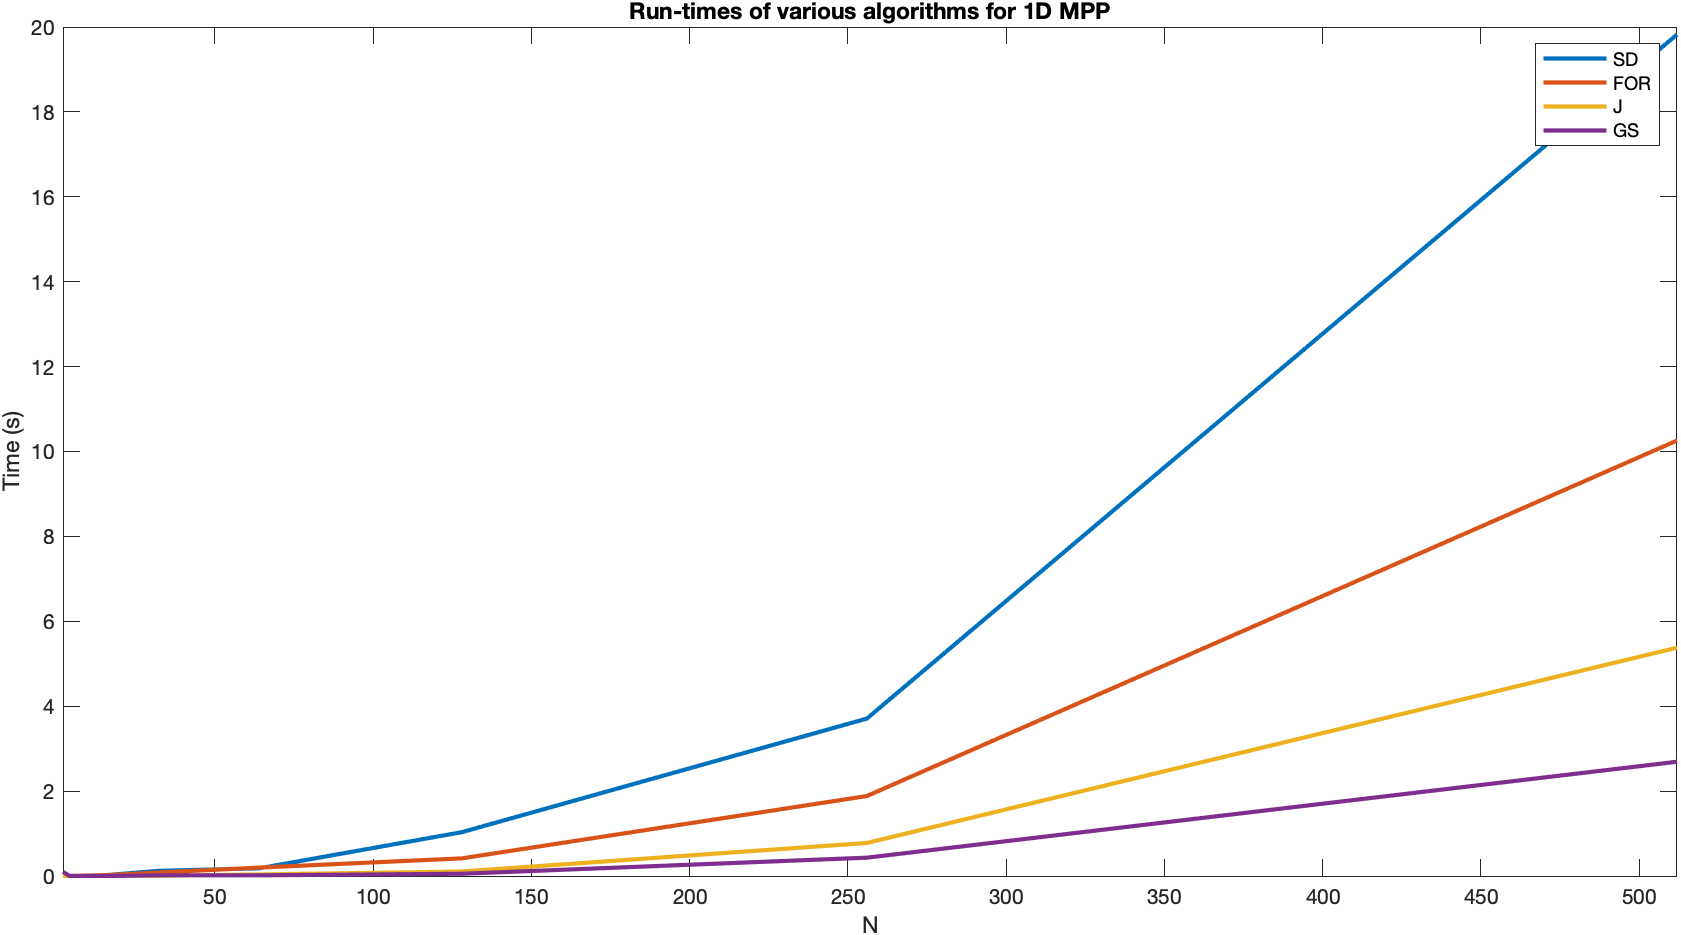
\includegraphics[width=15cm]{1Dtimes.png}\\
\it Times for $N\times N$ 1D MPP convergence for selected methods. Note each method is approximately a factor of two improvement.
\end{center}

\begin{center}
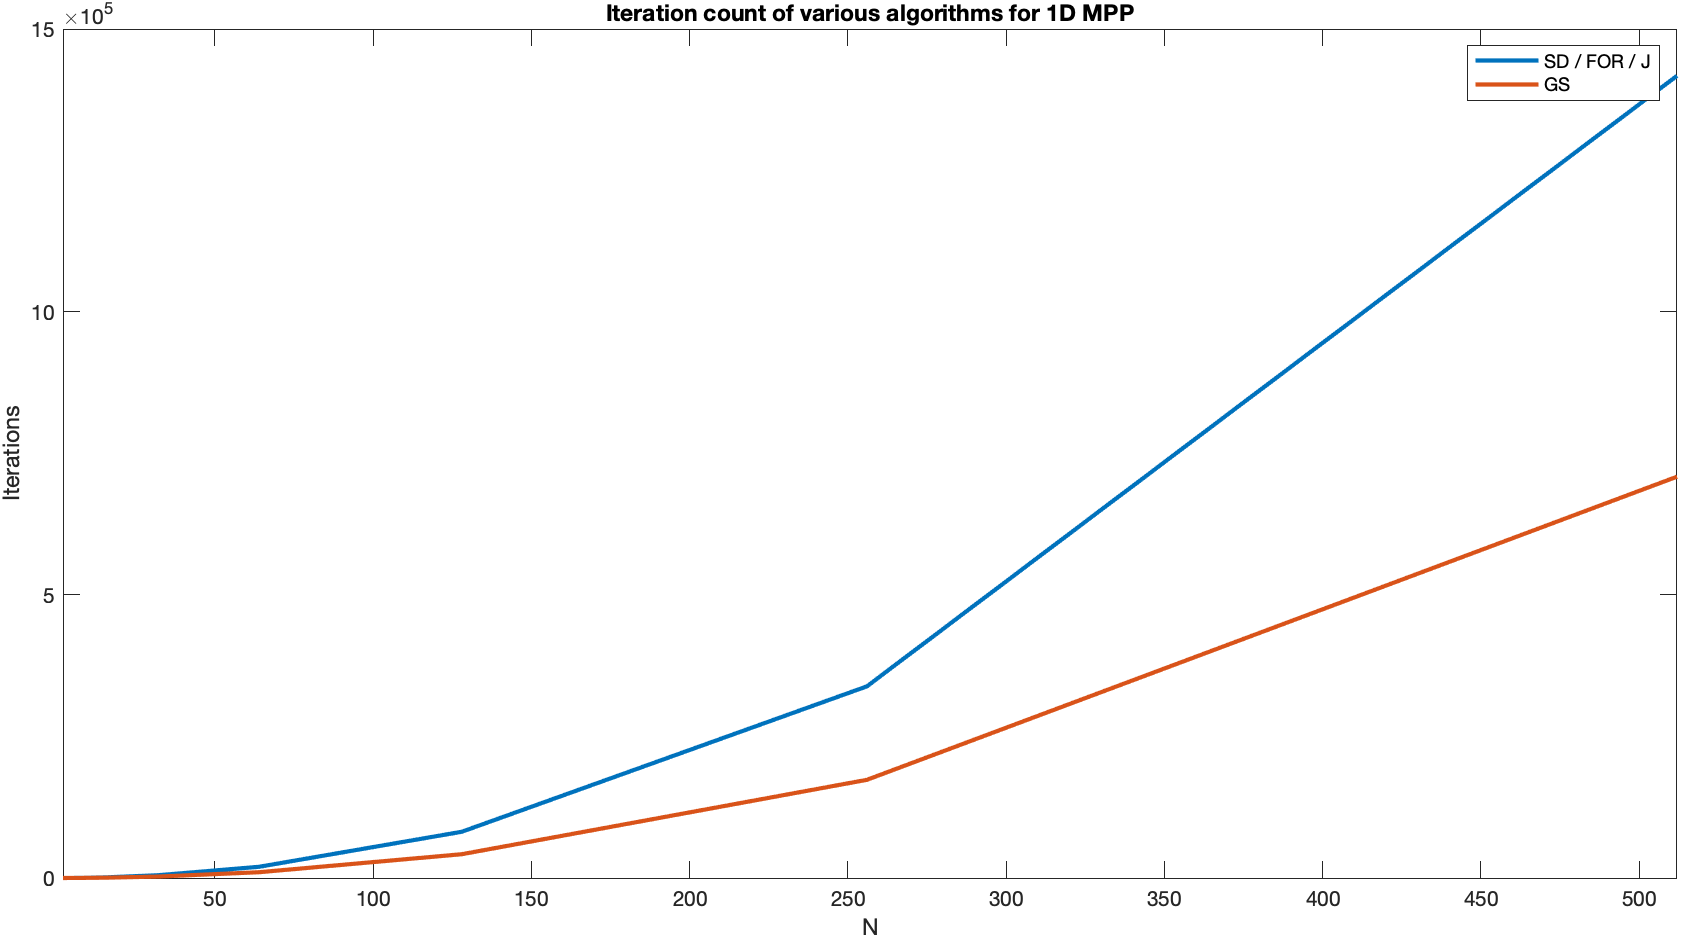
\includegraphics[width=15cm]{1Diters.png}\\
    \it Iterations for $N\times N$ 1D MPP convergence for selected methods. Note Steepest Descent, First Order Richardson, and the Jacobi method all took very similar amounts of iterations to converge.
\end{center}
We thus see the Jacobi method takes roughly the same number of iterations as the First Order Richardson or Steepest Descent, while the Gauss-Seidel method in this case takes roughly half the number of iterations. Indeed, there is no significant difference between the number of iterations for First Order Richardson, Steepest Descent, and the Jacobi method; at n = 512, FOR takes 1423600 iterations, SD takes 1412100, and Jacobi takes 1417300. Each iteration of the Jacobi method takes roughly half the time as the First Order Richardson and roughly a quarter of the time of Steepest Descent. Each iteration of the Gauss-Seidel method takes about the same time as an iteration of the Jacobi method (as we expect, since they do the same operations just with different values) as it completes half the iterations of the Jacobi method in half the time. Thus both the Jacobi and the Gauss-Seidel methods are better than Steepest Descent or First Order Richardson.
%\begin{center}
%\includegraphics[width=18cm]{1DIT.svg}
%\end{center}
%\begin{center}
%\includegraphics[width=18cm]{1DTI.png}
%\end{center}
%\subsubsection{Run-times}
%\begin{tabular}{lrrrr}
%\toprule
%     N    &       FOR (s)      &     SD (s)   &          GS (s)    &       J (s)\\    
 %    \midrule
  %  2   &     7.9397e-05   & 7.8984e-05    &      2.049e-05  &  0.00067294\\
   % 4   &   0.00044544   &  0.0007829    &     5.2909e-05   & 5.8247e-05\\
%    8   &    0.0017998   &  0.0038979    &       9.42e-05    &0.00018674\\
 %   16   &   0.0070002    &  0.012667    &     0.00066719  &  0.00077888\\
  %  32   &    0.046421     &  0.10312    &      0.0018499  &   0.0049358\\
   % 64   &      0.11377      & 0.20611    &       0.010102  &    0.017087\\
    %128  &     0.42793     &  0.82487    &       0.059637  &     0.11748\\
%    256  &     1.9808      &  3.8892    &        0.41043  &     0.76321\\
 %   512  &         10.637       & 19.105    &         2.7333  &      5.4184\\
  %  \bottomrule
%\end{tabular}

%\subsubsection{Iterations}
%\begin{tabular}{lrrrr}
%\toprule
%%    N   &       FOR       &     SD    &           GS     &       J     \\
  %  \midrule
   % 2     &         37     &       18        &       16    &        28\\
    %4     &        101  &          90         &      49     &       93\\
%    8     &        335   &        324          &    170      &     326\\
 %   16     &      1243    &      1240           &   639       &   1235\\
  %  32      &     4895     &     4936   &          2522        &  4887\\
   % 64       &   19857      &   20086    &        10225         &19849\\%
    %128       &  81673 &        82739     &       42006 &        81665\\
%    256 &   3.3839e+05  &  3.4194e+05      & 1.7342e+05  &  3.3853e+05\\
 %   512  &  1.4236e+06   & 1.4121e+06       &  7.09e+05   & 1.4173e+06\\
%\bottomrule
%\end{tabular}

%\subsubsection{Relative Error}
%\begin{tabular}{lrrrr}
%\toprule
%    N&          FOR   &         SD       &     GS   &         J     \\
%    \midrule
%    2 &     6.1508e-09&    1.8607e-09 &   4.0654e-10  &  3.7253e-09\\
%5    4  &    3.3088e-09 &   2.1366e-09  &  1.2044e-09   & 2.7322e-09\\
%    8   &   1.5008e-09  &  1.0684e-09   & 7.1401e-10    &1.5476e-09\\
%    16   &  6.1434e-10   & 4.3995e-10   & 3.0336e-10&     6.098e-10\\
%    32    & 2.3184e-10    &1.6525e-10   & 1.1541e-10 &   2.3124e-10\\
%    64    &  8.399e-11 &   6.0214e-11&    4.1911e-11  &   8.391e-11\\
%    128   & 3.0189e-11  &  2.1278e-11 &   1.5045e-11   & 3.0052e-11\\
%    256   & 1.0995e-11   & 7.8678e-12  &  5.6195e-12    &1.0331e-11\\
%    512   & 4.4157e-12    &3.1232e-12   & 3.0686e-12    &3.0973e-12\\
%    \bottomrule
%\end{tabular}


%\subsection{2D MPP}
\section{Conclusion}
While the Jacobi and Gauss-Seidel methods certainly have their merits - compared to Gaussian Elimination, our two iterative methods have superior run times - they also have faults of their own. For one, we are not guaranteed a usable result from either method unless the matrix satisfies the criteria laid out in section 2 of our paper. While there are a few other convergence criteria that we did not mention, there are still many cases where these methods fail to approximate the true solution. Also, when it comes to speed, faster methods exist, such as the Successive Over Relaxation method, which we briefly explore below. On the other hand, while the use of the Jacobi and Gauss-Seidel methods are today strictly academic, they do offer insight into iterative methods that are not dependent on the residual. These two methods are also important in that they can easily be performed by hand for small matrices, unlike other algorithms such as the Conjugate Gradient which, while more powerful, is truly meant for computer, not human, computation.  

Improvement for SOR comes from looking at the iterations displayed at the start of this paper (partially reproduced below) and noticing that  while the Jacobi method alternates between values lower and higher than the true solution, gradually narrowing in, the Gauss-Seidel method, after a few initial iterations, moves towards the true solution but remains on the same side (ie. it doesn't alternate).

\begin{center}
\begin{tabular}{llrrrrrrr}
\toprule
&&\multicolumn{6}{c}{Iteration}&\\\cline{3-8}
Method & entry & 0&1&2&3&4&5&True\\
\midrule
Jacobi & $x_1$ & 0 & .8571 & 1.2571 & .9611 & 1.1302 & .9257 & 1\\
Gauss-Seidel & $x_1$ & 0 & .8571 & 1.1803 & 1.0446 & 1.0089 & 1.0016 &1\\
\bottomrule
\end{tabular}
\end{center}

 Therefore we can make a significant improvement to the Gauss-Seidel method by making our iterative step some multiple of the Gauss-Seidel step. The relaxation factor must be between 0 and 2 to ensure convergence, although in practice would always be at least 1 in order to speed up, not slow down, the method \cite{Strang06}. The optimal relaxation factor can be determined with knowledge of the matrix' eigenvalues \cite{Strang06}. Although a simple idea, the results of this slight change can be impressive, with a single iteration of SOR often worth the equivalent of tens of iterations of the Jacobi method. This method is discussed in more detail in Strang's \textit{Linear Algebra} \cite{Strang06} and information about SOR is readily available both online and in other texts.



%%%%%%%%%%%%%%%%%%%%%%%%%%%%%%%%%%%%%%%%%%%%%%%%%%%%%%%%%%%%%%%%%%%%%%%%%%%%%%%%%%%%%%%%

\section*{Honor Code}
%%%%%%%%%%%%%%%%%%%% HONOR CODE and COLLABORATION PLEDGE %%%%%%%%%%%%%%%%%%%%%%%%%%%%%%
\begin{framed}
	\noindent \textbf{Honor Code Pledge:}\\  I have neither given nor received any unauthorized aide on this assignment. Daniel Ellison, DJ Poulin\\
	\noindent \textbf{Collaborative Work Pledge and Permission:}\\ I was an active collaborator on this assignment.  I approve of its final content. Daniel Ellison, DJ Poulin
	\vspace{1.5in}
\end{framed}
% The name of your bibfile.bib must appear here for this to work!
\nocite{*}
\bibliographystyle{plain}
\bibliography{bibfile.bib} 

\appendix
\section{Matlab Code}
\begin{algorithm}[Jacobi Method]
\begin{lstlisting}

function [xNew, i] = Jacobi(A, b, xOld, tol, itMax)
L = tril(A, -1);
LplusU = A - D;
bNorm = norm(b);
DInverse = inv(D);
LplusU = L + U;
for i = 1:itMax
    xNew = DInverse * (b - LplusU * xOld);
    xOld = xNew;
    relativeResidual = norm(b - A * xnew, 2) / bNorm;
    if  relativeResidual <= tol
        return
    end
end
end
\end{lstlisting}
\end{algorithm}

\begin{algorithm}[Gauss-Seidel]
\begin{lstlisting}

function [xNew, i] = GS(A, b, xOld, tol, itMax)
L = tril(A, -1);
U = A - tril(A);
D = diag(diag(A));
bNorm = norm(b);
LplusDInverse = inv(L + D);
for i = 1:itMax
    xNew = LplusDInverse * (b - U * xOld);
    xOld = xnew;
    relativeResidual = norm(b - A * xNew, 2) / bNorm;
    if  relativeResidual <= tol
        return
    end
end
end
\end{lstlisting}
\end{algorithm}
\end{document}